% Frames

% Rewriting => Giv et overview over de tools, konkret eksempel paa hvordan man implementerer det i et af tools'ene, kig paa hvilke features der er i hvert tool og stil det mere systematisk op end i rapporten

\begin{frame}{Rewriting}{}
\begin{block}{Automatic Code Rewriting}
	\begin{itemize}
		\item Useful for optimisation.
		\item Can be used to implement security features.
	\end{itemize}	
\end{block}
\end{frame}

\begin{frame}{Rewriting}{}
\begin{block}{Java Rewriting Tools}
\begin{align*}
BCEL && SERP && JTrek \\
ASM && Bit && JavaClass \\
Soot && Barista && Jalapeno \\
Sawja && Wala && JOIE
\end{align*}
\end{block}
\end{frame}

\begin{frame}[fragile]{Rewriting}{}
\begin{block}{Code Duplication}
\begin{lstlisting}[numbers=none, moredelim={[is][keywordstyle]{@@}{@@}}]                  
                        | ...
...	                | 17. push 0
15. load 6              | 19. if_cmpeq 33
17. push 0              | 21. load 6
19. if_cmpeq 25         | 23. push 0
...                     | 25. if_cmpeq 33
                        | ...
\end{lstlisting}  
\end{block}  
\end{frame}

\begin{frame}[fragile]{Rewriting}{}
\begin{block}{Code Duplication}
\begin{lstlisting}[numbers=none, moredelim={[is][keywordstyle]{@@}{@@}}]                  
...
11. add             
...	                          
17. load 10             
19. if_cmpeq 25        | if(b+c+... == e)
...                     
                     
\end{lstlisting}
\end{block}  
\end{frame}

\begin{frame}[fragile]{Rewriting}{}
\begin{block}{Sawja IR}
\begin{lstlisting}[numbers=none, moredelim={[is][keywordstyle]{@@}{@@}}]                  
...
0: $irvar0 := check() 
1: $irvar1 := getSig()
2: if ($irvar0) goto 4
...
\end{lstlisting}  
\end{block}  
\end{frame}

\begin{frame}{Rewriting}{}
\begin{figure}
  \centering
  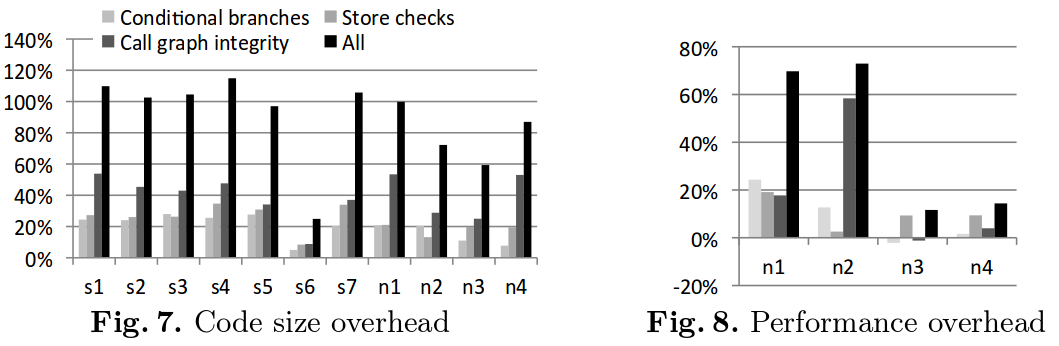
\includegraphics[width=\textwidth]{rewritingOverhead}
  \caption{Rewriting Overhead, Source: Mitigating Smart Card Fault Injection with Link-Time Code Rewriting: A Feasibility Study}
\end{figure}
\end{frame}

\begin{frame}[fragile]{Rewriting}{}
\begin{block}{Operand Stack Invariant}
\begin{lstlisting}[numbers=none, moredelim={[is][keywordstyle]{@@}{@@}}]                  
...                    | ...
1. @@pop@@                 | 1. dup
...                    | 2. @@pop@@
                       | 3. load 1
                       | 5. xor
                       | 6. store 1
                       | ...
                     
\end{lstlisting}
\end{block}  
\end{frame}
